% Svolgimento: prova del 01/02/1970, esercizio 3 -- shadowgraph del getto di un ugello a spina troncata piano.
% Numeri e figure: calcoli.py (stessa cartella). Compilare con: latexmk -pdf svolgimento.tex

\documentclass[11pt,a4paper]{article}

\usepackage[T1]{fontenc}
\usepackage[utf8]{inputenc}
\usepackage[italian]{babel}
\usepackage{amsmath,amssymb}
\usepackage[a4paper,margin=2.5cm]{geometry}
\usepackage{array}
\usepackage{siunitx}
\usepackage{booktabs}
\usepackage{graphicx}
\usepackage{float}
\usepackage{caption}
\usepackage{hyperref}

\hypersetup{hidelinks}
\setlength{\parindent}{0pt}
\setlength{\parskip}{4pt}
\allowdisplaybreaks
\graphicspath{{figure/}}
\sisetup{output-decimal-marker={,}, group-separator={\,}, per-mode=symbol,
         exponent-product=\cdot, range-phrase={\text{--}}}

\newcommand{\Cp}{C^{+}}
\newcommand{\Cm}{C^{-}}

\title{Gasdinamica -- Prova del 01/02/1970, esercizio 3\\[2pt]
\large Shadowgraph del getto di un ugello a spina troncata piano}
\author{}
\date{}

\begin{document}
\maketitle

\section*{Traccia}
\emph{Identificare le onde e le regioni numerate nella visualizzazione della corrente supersonica stazionaria generata
da un ugello a spina (plug) troncato bidimensionale} (Identify waves and regions numbered in the visualization of the
supersonic steady flow generated by a two-dimensional truncated plug nozzle; 4/30). Accanto allo shadowgraph c'è lo
schema della geometria (metà superiore). È la stessa traccia della prova del 25/01/2023.

%==============================================================================
\section{Lettura del testo e dell'immagine}
Lo schema mostra la metà superiore dell'ugello: una carenatura (cowl) con il bordo interno curvo, la gola fra il labbro
della carenatura e la sommità della spina, la rampa della spina che scende verso l'asse e il \textbf{troncamento}, cioè
una base piana perpendicolare all'asse. L'ugello è piano e simmetrico: lo shadowgraph mostra entrambe le metà, con
i due getti che escono dalle due fessure (labbri in alto e in basso a sinistra), il corpo nero della spina al centro e
la base sulla linea punteggiata verticale. La corrente va da sinistra verso destra.

Lo shadowgraph rende visibili le variazioni del \emph{gradiente} di densità: gli urti appaiono come coppie di linee
scura--chiara molto nette, gli strati di scorrimento come linee più sfumate, e le teste e le code dei ventagli
d'espansione, dove il gradiente di densità cambia bruscamente, come linee singole. Le strutture sono nitide e
ripetute simmetricamente: il campo è \textbf{stazionario}, come dice il testo.

Non ci sono scale né pressioni assegnate: le lunghezze le riferisco alla semialtezza della base $h_b$ e le pressioni
alla pressione totale in camera $p_0$; assumo aria, $\gamma=1{,}4$.

\begin{figure}[H]
  \centering
  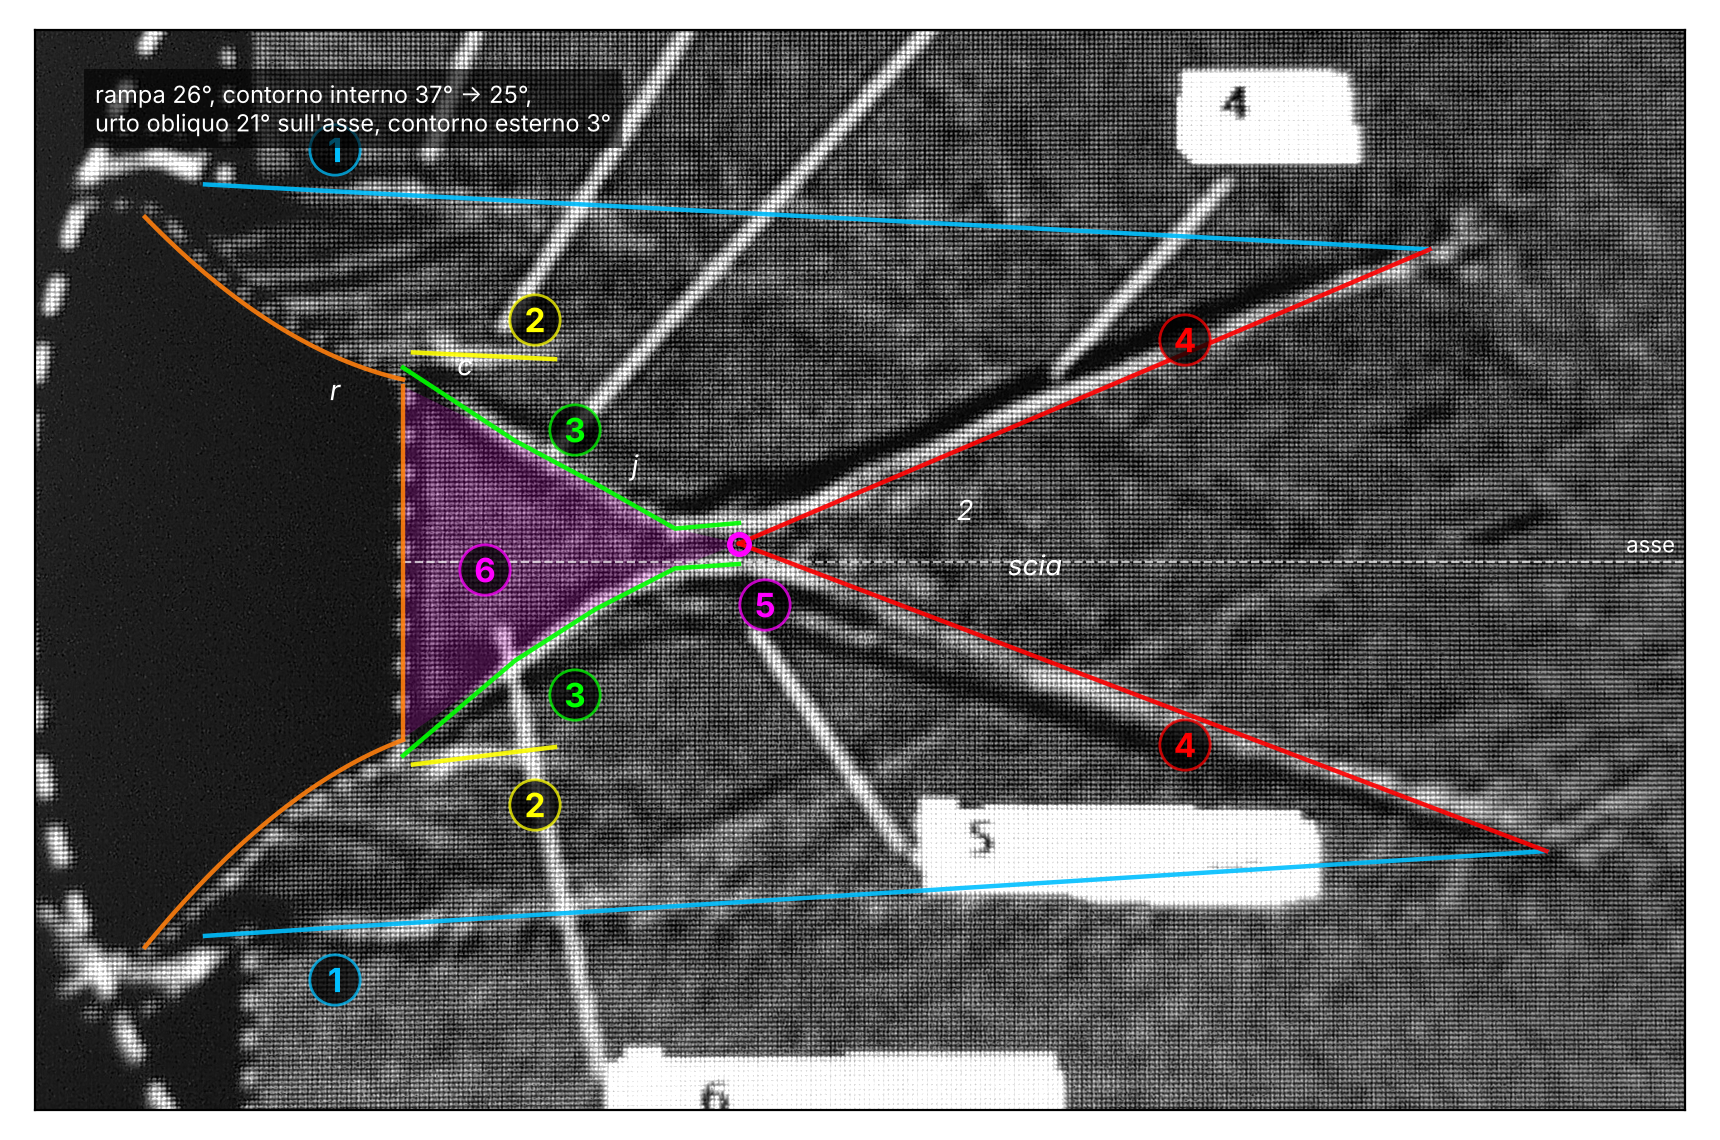
\includegraphics[width=0.92\textwidth]{annotata.png}
  \caption{Shadowgraph (raddrizzato) con le strutture identificate. Arancio: rampe della spina e base; ciano (1):
  contorni esterni del getto; giallo (2): linea che parte dallo spigolo della base; verde (3): contorni interni del
  getto; rosso (4): urti obliqui di ricompressione; magenta: punto di ristagno al collo (5) e regione di base (6). Le
  lettere $r$, $c$, $j$, 2 indicano gli stati della metà superiore.}
  \label{fig:ann}
\end{figure}

%==============================================================================
\section{Identificazione delle strutture}
Nell'ordine dei numeri (fig.~\ref{fig:ann}); le strutture della metà inferiore sono le speculari.
\begin{enumerate}
\item \textbf{Contorno esterno del getto} (jet boundary). Parte dal labbro della carenatura e separa il getto
  dall'aria ambiente in quiete: è una \textbf{superficie libera}, cioè uno strato di scorrimento su cui la pressione
  vale $p_a$ e la velocità è tangente; per viscosità diventa uno strato di mescolamento che si allarga verso valle.
  È quasi rettilineo e quasi parallelo all'asse. Fra il labbro e la rampa c'è il ventaglio d'espansione centrato nel
  labbro (onde $\Cm$, striature fra 1 e la rampa), che porta la corrente esterna alla pressione ambiente: è
  l'espansione esterna tipica della spina, quella che le permette di adattarsi alla quota.
\item \textbf{Struttura allo spigolo della base} (il «labbro» della base, lip). Nello spigolo la corrente della rampa
  gira verso l'asse per adattarsi alla pressione della regione di base: nasce un \textbf{ventaglio d'espansione
  centrato} (onde $\Cp$), e a ridosso dello spigolo, nello strato limite che si stacca, un urto debole di
  ricompressione, il \textbf{lip shock}. La linea visibile, corta e un po' curva, ha l'inclinazione della testa del
  ventaglio (la verifico nel calcolo); il lip shock non si distingue da essa.
\item \textbf{Contorno interno del getto} (inner jet boundary). Strato di scorrimento che parte dallo spigolo e
  separa il getto dalla regione di base ricircolante; è il prolungamento \emph{fluido} della spina troncata. È
  \textbf{curvo}: scende verso l'asse sempre meno inclinato, quindi ruota la corrente in senso antiorario e la
  comprime con onde $\Cp$ che coalescono nell'urto 4.
\item \textbf{Urto obliquo di ricompressione} (trailing shock). Parte dal collo, dove i due contorni interni si
  incontrano, e risale verso il contorno esterno: è della famiglia $\Cp$ e raddrizza parallelamente all'asse la
  corrente che convergeva verso di esso (le due metà si comportano come una riflessione regolare sull'asse). È la
  linea più netta della figura, con la coppia scura (a monte)--chiara (a valle) tipica dell'urto.
\item \textbf{Punto di ristagno posteriore della scia chiusa} (collo). I due contorni interni si chiudono sull'asse:
  la linea di corrente che separa il fluido del getto da quello ricircolante arriva sull'asse con velocità nulla,
  perché la ricompressione dell'urto 4 non lascia proseguire il fluido lento dello strato di scorrimento, che viene
  rimandato verso la base. Da qui partono i due urti 4 e, fra di essi, la \textbf{scia} lungo l'asse.
\item \textbf{Scia chiusa} (closed wake): la \textbf{regione di base}, delimitata dalla base e dai contorni
  interni fino al collo. Il fluido vi ricircola lentamente (subsonico) a pressione quasi uniforme $p_b$, la
  \textbf{pressione di base}. È «chiusa» perché è circondata da corrente supersonica: non comunica con l'ambiente. È
  una \textbf{poppa fluida} che sostituisce la parte di spina tolta con il troncamento.
\end{enumerate}
Sono invece artefatti il reticolo fine (foto dello schermo), i puntini che disegnano il contorno della spina e la
cornice della finestra, e le linee bianche dei rimandi ai numeri.

%==============================================================================
\section{Ipotesi e modello}
\begin{itemize}
\item \textbf{Corrente supersonica fuori dalla regione di base e dalla scia.} Lo dicono gli urti obliqui netti (4) e
  i ventagli centrati negli spigoli, che esistono solo in corrente supersonica; il testo lo conferma. Uso quindi il
  modello \textbf{2D stazionario supersonico} (ventagli di Prandtl--Meyer, urti obliqui, caratteristiche $\Cp$ e
  $\Cm$) nei getti, e la regione di base come regione a pressione uniforme $p_b$.
\item \textbf{Corrente isentropica dalla camera fino all'urto 4}, con $p_0$ uniforme sulla linea di corrente che
  costeggia il contorno interno: trascuro il lip shock, che è debole.
\item \textbf{Contorni come condizioni al contorno}: sul contorno esterno $p=p_a$; sul contorno interno $p=p_b$
  vicino allo spigolo e direzione della corrente uguale a quella del contorno (che misuro sull'immagine).
\item \textbf{Simmetria}: calcolo la metà superiore e uso, per gli angoli, le medie delle due metà, che differiscono
  di pochi gradi.
\end{itemize}

%==============================================================================
\section{Misure sull'immagine}
Con righello e goniometro, prendendo l'asse come la mezzeria fra i due spigoli della base (angoli misurati dall'asse,
verso l'asse se non detto altrimenti):
\begin{itemize}
\item rampa della spina, nel tratto finale: \textbf{\ang{26}} (più ripida a monte, circa \ang{45});
\item contorno interno (3): \textbf{\ang{37}} subito dopo lo spigolo, \ang{32} a metà, \textbf{\ang{25}} prima del
  collo;
\item linea allo spigolo (2): circa \ang{5};
\item urto obliquo (4): \textbf{\ang{21}} sull'asse, verso l'esterno;
\item contorno esterno (1): circa \ang{3};
\item collo (5) a distanza $L\approx1{,}9\,h_b$ dalla base; gli urti 4 arrivano sui contorni esterni a circa
  $6\,h_b$ dalla base.
\end{itemize}

%==============================================================================
\section{Analisi qualitativa e topologia}
\begin{figure}[H]
  \centering
  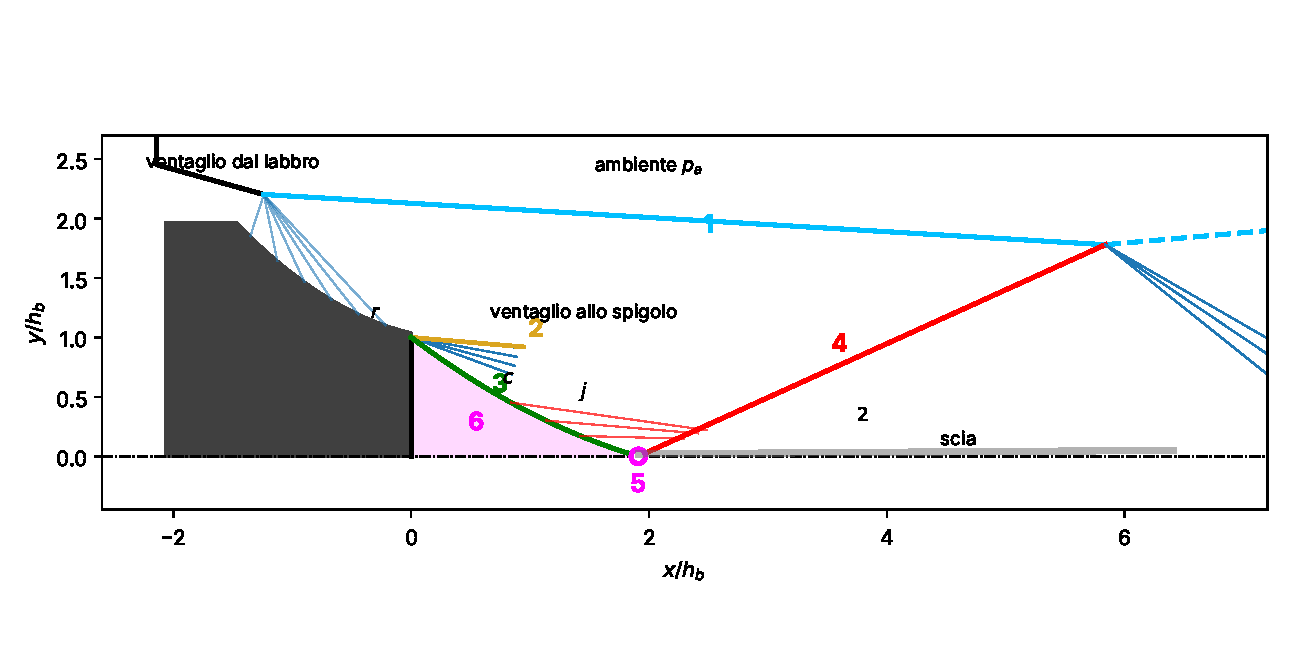
\includegraphics[width=0.92\textwidth]{schema.pdf}
  \caption{Schema della metà superiore in unità di $h_b$, con le strutture 1--6, i ventagli (blu), le onde di
  compressione del contorno interno (rosso sottile) e l'espansione in cui l'urto 4 si riflette sul contorno esterno.}
  \label{fig:schema}
\end{figure}
Seguo una linea di corrente vicina al contorno interno della metà superiore (fig.~\ref{fig:schema}):
\begin{itemize}
\item lungo la rampa la corrente espande (stato $r$ alla fine della rampa, inclinata di \ang{-26});
\item nello spigolo la pressione di base è minore di quella di fine rampa, quindi la corrente gira verso l'asse
  attraverso il ventaglio centrato $\Cp$ (2) fino alla direzione iniziale del contorno interno, \ang{-37}: stato $c$,
  alla pressione $p_b$;
\item lungo il contorno interno curvo la corrente viene raddrizzata gradualmente da onde di compressione $\Cp$ fino a
  \ang{-25}: stato $j$, subito prima dell'urto;
\item al collo l'urto obliquo $\Cp$ (4) la porta parallela all'asse: stato 2, che è anche lo stato della metà
  inferiore per simmetria.
\end{itemize}
Più all'esterno la corrente non attraversa l'urto vicino al collo ma più a valle; l'urto arriva sul contorno esterno e,
poiché lì la pressione è imposta ($p_a$), si riflette come espansione $\Cm$ e il contorno piega verso l'esterno:
comincia la struttura a celle del getto. Le zone a due famiglie (onde del labbro riflesse dalla rampa, onde di
compressione che attraversano il ventaglio dello spigolo) non le risolvo: le tratto come regioni di raccordo fra gli
stati uniformi.

\begin{table}[H]
  \centering
  \small
  \begin{tabular}{cp{6.6cm}p{5.4cm}}
    \toprule
    Stato & Posizione & Come lo si raggiunge \\
    \midrule
    $r$ & corrente sulla rampa, allo spigolo & espansione isentropica dalla gola \\
    $c$ & dopo il ventaglio dello spigolo, lungo il contorno interno; $p=p_b$ & ventaglio $\Cp$ (2) \\
    $j$ & lungo il contorno interno, prima del collo & compressione isentropica $\Cp$ \\
    2 & dietro l'urto 4, corrente assiale & urto obliquo $\Cp$ (4) \\
    $b$ & regione di base (6), quasi ferma, $p=p_b$ & contorno interno (3) \\
    $a$ & ambiente, $p=p_a$ & contorno esterno (1) \\
    \bottomrule
  \end{tabular}
  \caption{Stati della metà superiore (la metà inferiore è speculare: $r'$, $c'$, $j'$).}
\end{table}

%==============================================================================
\section{Calcolo}

\subsection*{a) Urto 4: numero di Mach a monte ($j\to2$)}
La corrente a monte è inclinata come il contorno interno prima del collo, a valle è assiale: la deviazione è
$\theta=\ang{25}$. L'urto forma \ang{21} con l'asse dalla parte opposta, quindi con la corrente a monte forma
$\sigma=\ang{21}+\ang{25}=\ang{46}$. Dalla relazione $\theta$--$\sigma$--$M$
\[
\tan\theta=2\cot\sigma\,\frac{M^2\sin^2\sigma-1}{M^2(\gamma+\cos2\sigma)+2}
\]
si ricava $M$ in forma esplicita (è lineare in $M^2$):
\[
M_j^2=\frac{2(\tan\theta+\cot\sigma)}{2\cot\sigma\sin^2\sigma-\tan\theta\,(\gamma+\cos2\sigma)}
\quad\Rightarrow\quad M_j\approx2{,}8 .
\]
Attraverso l'urto, con le relazioni dell'urto normale applicate alla componente normale:
\[
M_{n,j}=M_j\sin\sigma\approx2{,}02,\qquad
\frac{p_2}{p_j}=1+\frac{2\gamma}{\gamma+1}\left(M_{n,j}^2-1\right)\approx4{,}6,
\]
\[
M_{n2}^2=\frac{1+\delta M_{n,j}^2}{\gamma M_{n,j}^2-\delta},\qquad
M_2=\frac{M_{n2}}{\sin(\sigma-\theta)}\approx1{,}6,\qquad \frac{p_{02}}{p_{0}}\approx0{,}71 .
\]

\subsection*{b) Contorno interno: stati $c$ e $r$}
Il ventaglio dello spigolo e le compressioni del contorno curvo sono onde $\Cp$ (nascono dal contorno, che sta sotto
la corrente della metà superiore): attraverso di esse si conserva l'invariante delle $\Cm$,
\[
\theta+\nu=\text{cost}\quad\Rightarrow\quad
\nu_c=\nu_j+\theta_j-\theta_c,\qquad \nu_r=\nu_j+\theta_j-\theta_r .
\]
Con $\nu_j=\nu(M_j)\approx\ang{45.9}$, $\theta_j=\ang{-25}$, $\theta_c=\ang{-37}$, $\theta_r=\ang{-26}$:
\[
\nu_c\approx\ang{57.9}\ \Rightarrow\ M_c\approx3{,}5,\qquad
\nu_r\approx\ang{46.9}\ \Rightarrow\ M_r\approx2{,}9 .
\]
Le pressioni seguono dall'isentropica, $p/p_0=(1+\delta M^2)^{-\gamma/(\gamma-1)}$:
\[
\frac{p_r}{p_0}\approx0{,}034,\qquad \frac{p_b}{p_0}=\frac{p_c}{p_0}\approx0{,}014,\qquad
\frac{p_j}{p_0}\approx0{,}036,\qquad \frac{p_2}{p_0}=\frac{p_2}{p_j}\frac{p_j}{p_0}\approx0{,}17 .
\]
Quindi $p_b/p_r\approx0{,}41$: la pressione di base è circa il 40\% di quella di fine rampa, e la ricompressione al
collo la moltiplica per circa 12 ($p_2/p_b\approx12$).

\subsection*{c) Testa e coda del ventaglio dello spigolo}
Per un ventaglio centrato $\Cp$ testa e coda sono inclinate di $\theta+\mu$, con $\mu=\arcsin(1/M)$:
\[
\theta_r+\mu_r\approx\ang{-26}+\ang{20.5}=\ang{-5.5},\qquad
\theta_c+\mu_c\approx\ang{-37}+\ang{16.8}=\ang{-20} .
\]

%==============================================================================
\section{Verifiche}
\begin{enumerate}
\item Urto 4 sul ramo debole: $\theta=\ang{25}<\theta_{\max}(2{,}8)=\ang{32.7}$ e $\sigma=\ang{46}$ minore dell'angolo
  del punto di $\theta_{\max}$ (\ang{65}); come atteso in campo aperto. \emph{Verificata.}
\item Corrente dietro l'urto supersonica, $M_2\approx1{,}6$: il modello 2D stazionario vale anche a valle del collo
  (fuori dalla scia). \emph{Verificata.}
\item Entropia: $p_{02}/p_0\approx0{,}71<1$, $\Delta s>0$; l'urto è di compressione ($p_2>p_j$). \emph{Verificata.}
\item Natura delle onde: allo spigolo la corrente ruota verso l'asse (da \ang{-26} a \ang{-37}), cioè $\theta$
  diminuisce attraverso onde $\Cp$: espansione, $p_b<p_r$; lungo il contorno interno $\theta$ aumenta: compressione,
  coerente con l'urto 4 che ne è la coalescenza. \emph{Verificata.}
\item La linea 2 è la testa del ventaglio dello spigolo: inclinazione prevista \ang{-5.5}, misurata circa \ang{-5}.
  \emph{Verificata}; la coda (\ang{-20}) non si vede perché le compressioni del contorno curvo la attraversano subito.
\item Geometria della scia chiusa: l'inclinazione media del contorno interno fra spigolo e collo,
  $\arctan(h_b/L)\approx\ang{28}$, sta fra quella iniziale (\ang{37}) e quella finale (\ang{25}).
  \emph{Coerente.}
\end{enumerate}

%==============================================================================
\section{Risultati}
\begin{table}[H]
  \centering
  \small
  \begin{tabular}{clp{7.2cm}}
    \toprule
    N. & Struttura & Natura \\
    \midrule
    1 & contorno esterno del getto & superficie libera (strato di scorrimento) a $p=p_a$, dal labbro della carenatura \\
    2 & struttura allo spigolo della base & ventaglio d'espansione $\Cp$ centrato nello spigolo (se ne vede la testa),
        con il lip shock a ridosso dello spigolo \\
    3 & contorno interno del getto & strato di scorrimento curvo fra getto e regione di base, a $p_b$ vicino allo
        spigolo \\
    4 & urto obliquo di ricompressione & urto $\Cp$ dal collo, raddrizza la corrente lungo l'asse \\
    5 & punto di ristagno al collo & chiusura della scia: i contorni interni si incontrano sull'asse \\
    6 & scia chiusa (regione di base) & ricircolazione subsonica a pressione uniforme $p_b$ (poppa fluida) \\
    \bottomrule
  \end{tabular}
  \caption{Identificazione delle strutture numerate.}
\end{table}

\begin{table}[H]
  \centering
  \begin{tabular}{cccc}
    \toprule
    Stato & $\theta$ & $M$ & $p/p_0$ \\
    \midrule
    $r$ (fine rampa) & \ang{-26} & $\approx2{,}9$ & $\approx0{,}034$ \\
    $c$ (dopo lo spigolo) & \ang{-37} & $\approx3{,}5$ & $\approx0{,}014=p_b/p_0$ \\
    $j$ (prima del collo) & \ang{-25} & $\approx2{,}8$ & $\approx0{,}036$ \\
    2 (dietro l'urto 4) & \ang{0} & $\approx1{,}6$ & $\approx0{,}17$ \\
    \bottomrule
  \end{tabular}
  \caption{Stati lungo il contorno interno della metà superiore (valori stimati dalle misure).}
\end{table}

%==============================================================================
\section{Rappresentazioni}
\begin{figure}[H]
  \centering
  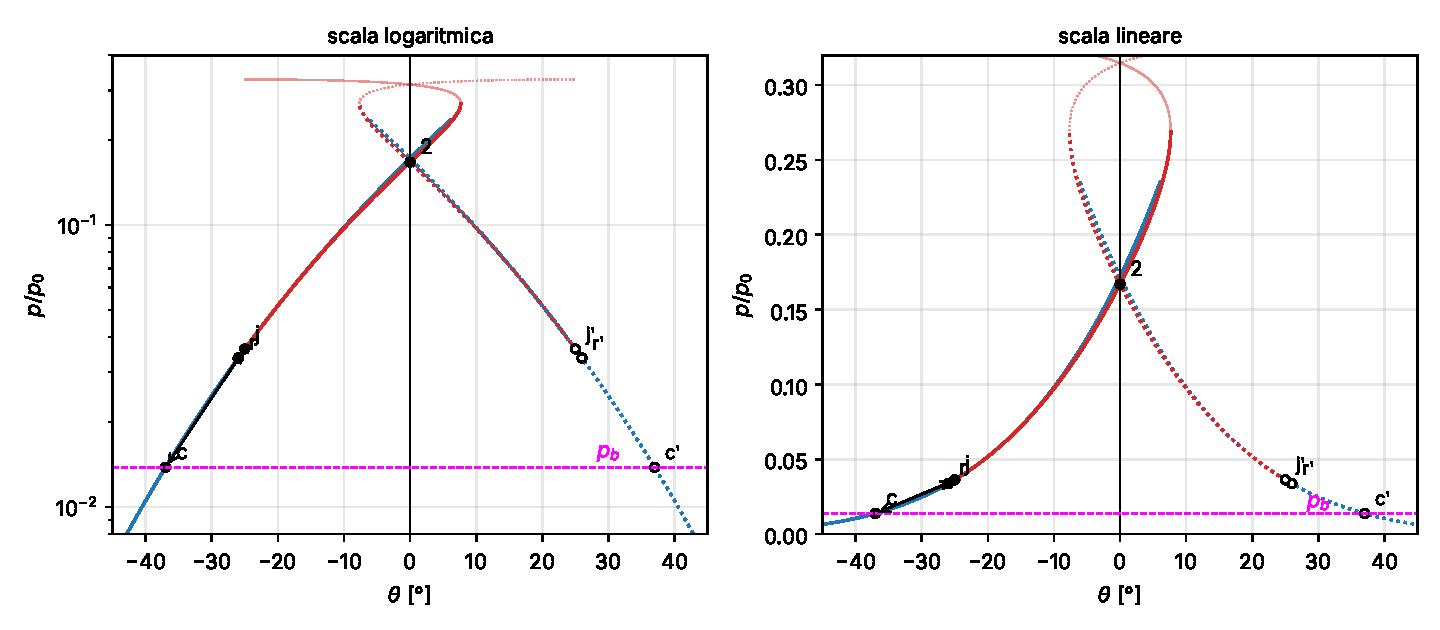
\includegraphics[width=\textwidth]{p_theta.pdf}
  \caption{Piano $p$--$\theta$ (pressioni riferite a $p_0$): curva isentropica $\Cp$ per $r$, $c$, $j$ (blu), polare
  $\Cp$ di $j$ (rosso; sottile il ramo forte), le stesse curve speculari per la metà inferiore (punteggiate) e la
  pressione di base $p_b$.}
  \label{fig:pth}
\end{figure}
\textbf{Piano $p$--$\theta$} (fig.~\ref{fig:pth}). Gli stati $r$, $c$, $j$ stanno sulla stessa curva isentropica,
perché il ventaglio dello spigolo e le compressioni del contorno interno sono onde della stessa famiglia $\Cp$: la
corrente scende da $r$ a $c$ (espansione fino a $p_b$, la retta tratteggiata) e risale fino a $j$. Dalla polare $\Cp$
di $j$ il ramo debole porta a $\theta=0$ nello stato 2; la polare speculare della metà inferiore passa per lo stesso
punto: le due correnti si raccordano sull'asse con la stessa pressione e la stessa direzione, come in una riflessione
regolare. Le pressioni vanno da $0{,}014\,p_0$ a $0{,}17\,p_0$, un ordine di grandezza: la scala logaritmica mostra
bene la zona di bassa pressione intorno a $r$, $c$, $j$ (dove la scala lineare schiaccia gli stati sull'asse delle
ascisse), quella lineare dà la proporzione reale del salto di pressione all'urto, molto maggiore delle variazioni lungo
il contorno interno.

%==============================================================================
\section{Coerenza con l'immagine e discussione}
\begin{itemize}
\item Il modello ritrova le strutture visibili: la testa del ventaglio dello spigolo ha l'inclinazione della linea 2,
  il contorno interno curvo con le compressioni che coalescono nell'urto 4, l'urto sul ramo debole che lascia una
  corrente supersonica parallela all'asse. Più a valle si intravedono le onde che nascono dalla riflessione degli urti
  4 sui contorni esterni e si incrociano vicino all'asse: è l'inizio della struttura a celle del getto.
\item \textbf{Scia chiusa e pressione di base.} La regione di base è racchiusa da corrente supersonica, quindi
  l'ambiente non vi può far arrivare informazione: $p_b/p_0$ non dipende da $p_a$ e resta fissata dal campo del getto
  (qui circa $0{,}014$). Il contorno esterno invece è a $p_a$ e si adatta alla quota: è il vantaggio della spina
  rispetto a un ugello a campana. A rapporti di pressione più bassi la scia è \emph{aperta}: la regione di base
  comunica con l'ambiente attraverso una scia subsonica e $p_b$ segue $p_a$.
\item \textbf{Poppa fluida.} La scia chiusa fa da prolungamento fluido della spina: il contorno interno, curvo da
  \ang{37} a \ang{25}, prende il posto della parte di rampa tolta, che avrebbe ruotato la corrente fino alla
  direzione assiale con un'espansione senza urti. Con il troncamento la ricompressione finale avviene invece con
  l'urto 4, con una perdita di pressione totale (circa il 30\% sulla linea di corrente vicina al contorno interno) e
  una base a pressione minore di quella di fine rampa, che sulla base produce una spinta ridotta.
\item \textbf{Limiti del modello.} Gli strati di scorrimento hanno spessore finito e crescono verso valle (il collo è
  in realtà una zona di dimensione finita, non un punto); il lip shock nasce nello strato viscoso e non è descritto
  dal modello non viscoso; la ricompressione al collo è distribuita fra onde e urto. Per $M$ elevati $\nu(M)$ varia
  poco, quindi $M_c\approx3{,}5$ e $p_b$ sono solo indicativi; $M_j$, ricavato direttamente dall'urto, è la stima più
  robusta.
\end{itemize}

\end{document}
